\documentclass[11pt]{article}
\usepackage{amsmath}
\usepackage{graphicx}
\begin{document}
\section{Introduction}

The experiment consists of a microwave cavity in the bore of a superconducting solenoid magnet from Cryo Industries. The bore diameter is 89 mm and the cryostat housing the cavity is 1and5/8” dia. wide. The cryostat is offset from the bore center so that there is enough space for a second cavity to sit in the bore, outside the cryostat. There are two cryogenic amplifiers with a gain of 50 dB and waveguides WR28 carry the signal power out of the cryostat to a room temperature electronics chain which filters, amplifies, and mixes the signal down to baseband, so it can be digitized. We have a PCI- National Instruments (PCI-5114) digitizer that samples at a rate of 10 MHz second, with a 10 MHz digital signal sent in by the PXA Signal Analyzer (GET MODEL NUMBER) which is in turn phase locked to the first signal generator, which outputs a 10 MHz analog signal. A test tone signal is generated by a second signal generator, also an ANRITSU MG3694C, offset to 3 MHz lower than the cavity resonant frequency. There is an RF switch (model number) to connect either one cable of the network analyzer (also frequency locked) or to take the signal power to the receiver. There is another RF switch on the other cable of the network analyzer that connects either the test tone signal to the calibration port or the network analyzer input. 

SCHEMATIC OF EXPERIMENT

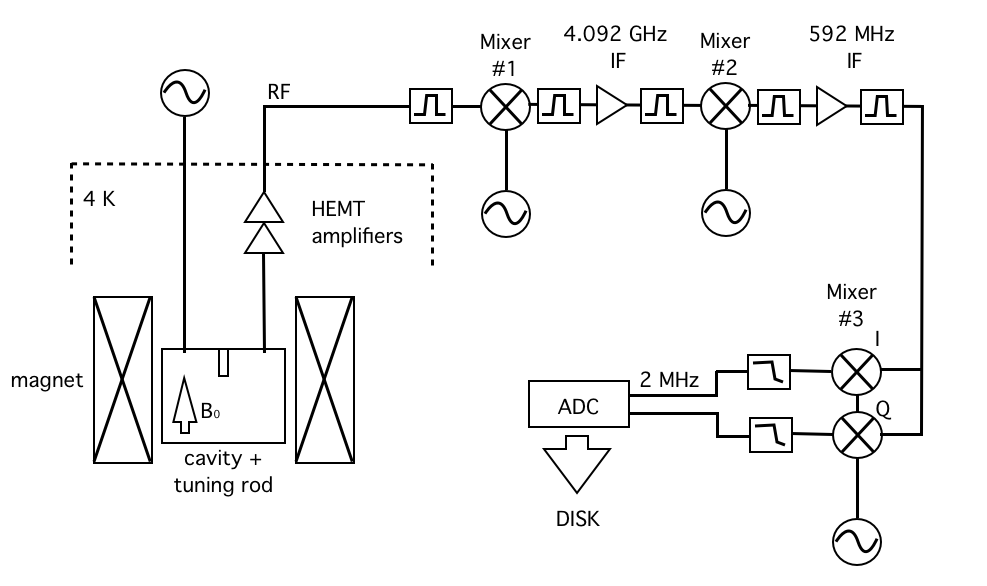
\includegraphics[width=\textwidth]{schematicnew}

\section{The Magnet}

The magnet is a NbTi alloy with copper windings. It is superconducting. It is made by Oxford instruments. It is run in persistent mode. The helium consumption is 10 L$/$day. The bore is warm and has a dia. of 89 mm.
Over the size of the cavity we predict that the magnetic field will be constant and so it is.

I should get an nmr hall probe. Check e-bay.

The magnetic field is 7 Tesla. The magnet was cooled in the spring or maybe the summer of 2011. 

PICTURE OF THE MAGNET
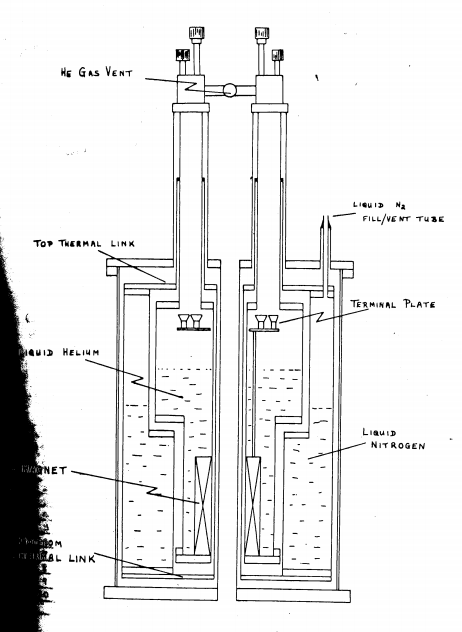
\includegraphics[width=\textwidth]{nmrmagnet}

\section{The MIcrowave Cavity}

The cavity is a right circular cylinder made of OFHC copper. The cavity has two aperture couplings on the side - these apertures go to WR28 waveguide, which is soldered on. The cavity has a removable bottom lid, which can be screwed on with HOW MANY? 2-56 screws with Belleville washers - it has a groove for an indium seal, with the outer lip of the groove tapered off. This ensures the contact happens between the inner lip of the groove and the cavity bottom.

PICTURE OF ENGINEERING DRAWING OF CAVITY
\begin{figure}
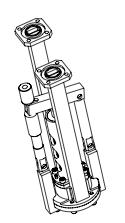
\includegraphics[scale=1.4]{AxionDrawing3D}
\end{figure}

\begin{figure}
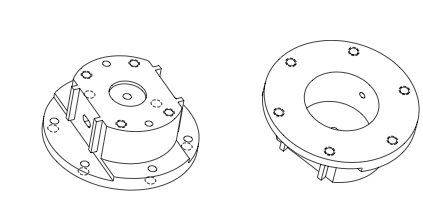
\includegraphics[scale=0.7]{AxionBody}
\end{figure}

\begin{figure}
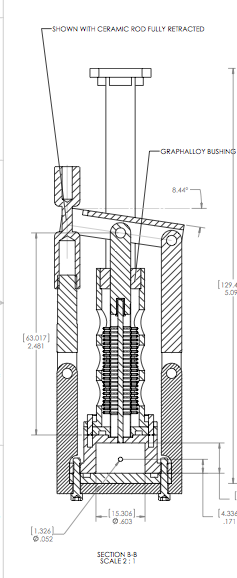
\includegraphics[scale=0.7]{AxionEngineeringDrawing}
\end{figure}

The walls of the cavity are 40 thousandths thick at their thinnest point. There is a small hole for the weak coupling port and a large oval “racetrack” hole for the strong port.  The cavity was simulated in Ansoft HFSS. I took the surface roughness into account but eventually took it out because it did not make a difference. 

PICTURE OF HFSS SIMULATION OF CAVITY WITH ™020 MODE E FIELD

Two cavities were made - the difference between them being that the small hole was .052” or .05”, and that the length between the center of the hole and the ledge on which the waveguides rested was .06” or .08”. Both of these parameters should have given equivalent cavities, but when tested, it was seen that the first cavity had a worse Q (it had a rougher finish) but was also much more overcoupled. HOwever, the loss through the weak port was -50 dB as expected. The second cavity had a higher Q, was less overcoupled (although still slightly overcoupled), but had a much higher loss of -60 dB. We performed several tests with different bottom lids, cooling the cavitiy in an open nitrogen dewar, and also running helium gas through the system to prevent ice from forming. The results of the tests were that at 77 K, the loaded Q and betas of cavity 1 and two are THIS and THAT. The second cavity was cleaned after the waveguides were soldered on, and there was a rouge polishing applied to get the cavity finish to be good. THe theoretical Q expected is WHAT.

THEORETICAL UNLOADED Q for TM0m0 modes: from Roger's thesis
"
$$Q_0 = \frac{\mu}{\mu_c} (\frac{\mu_c \omega \sigma}{2})^{1/2} \frac{V}{S} \cdot 2 $$

$\mu$ and $\mu_c$ are the permeabilities of the cavity interior and walls in MKS units, which are nearly equal to $\mu_0$ for helium and copper: $\omega$ is the resonant frequency and $\sigma$ the conductivity of the walls.

$\sigma = 5.86 \times 10^{7}/\Omega\cdot\text{cm}$ for oxygen-free copper at 294 K."

PLOT OF EXPECTED Q VS TUNING AND ACTUAL Q VS TUNING
\begin{figure}
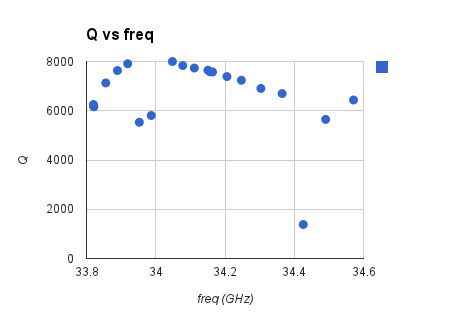
\includegraphics[scale=0.7]{Q_vs_freq}
\caption{TE011 mdoe Q tuning}
\end{figure}

\begin{figure}
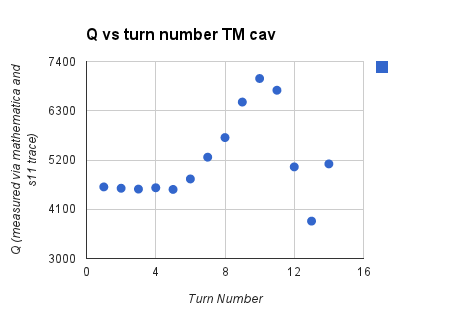
\includegraphics[scale=0.7]{TM_cav_Q_vs_turn_number}
\caption{TM Mode Q tuning}
\end{figure}


Although it is impossible to perform the same test with the cavity in situ because we cannot make a reflection measurement on the strong port (we don’t have space to put in a directional coupler), we see that the loaded Q is THIS at 4 K. 

PLOT OF SIMULATED FREQ COLD AND ACTUAL FREQ COLD

The simulation predicts that going from warm to cold, the thermal contraction taken into account and keeping the conductivity the same, that you should get so much change in the coupling and frequency.

The simulation predicts that you can tune over a XXX frequency range without a mode crossing. It also predicts that the Q should degrade by YYY over a certain range. The form factor is predicted to be ZZZ. What we see in practice is that there is a mode crossing (warm); in situ, there is a blind spot. The upper and lower modes should be TE112 and TM010.

PLOT OF TUNING FOR TE011 mode cavity
\begin{figure}
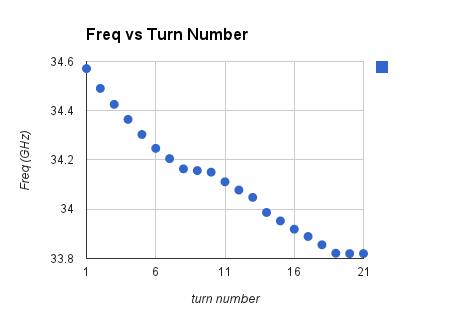
\includegraphics[scale=0.7]{freq_vs_turn_number}
\caption{TE mode freq tuning}
\end{figure}

We tune using a 1/16th inch thick dielectric rod ordered from McMaster, with the suppliers originally being Coorstek. THis alumina rod is secured with a socket used for electronics work which is soldered to a copper top hat. This has a groove for an indium seal and this hat is screwed on to the top face of the cavity. There is a small beryllium copper bellows soldered on to the top of the top hat, and this is encased in a tube which provides structural support to make sure the bellows only has one degree of freedom in the vertical direction. 

There is a lever arm that pushes the bellows up or down - this is controlled by a G-10 tube that connects from a screw at the top of the cryostat which we manually turn, and thus allows us to translate the rotation motion into translational motion of the lever arm. 

PICTURE OF INSERT
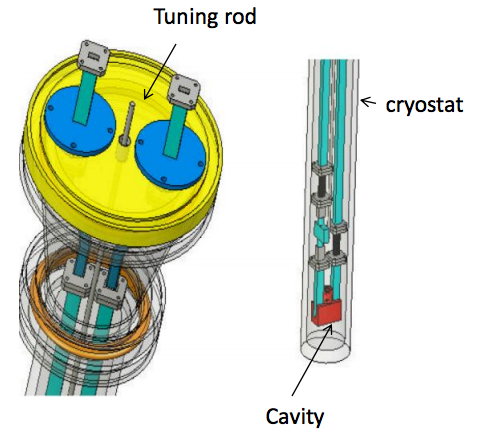
\includegraphics[width=\textwidth]{insertdrawing}
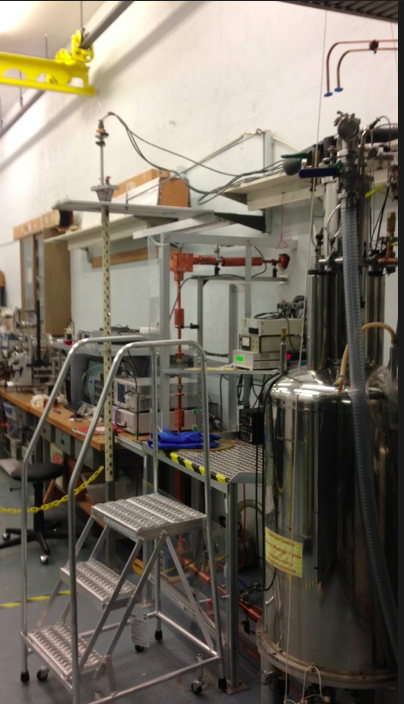
\includegraphics[width=\textwidth]{experiment}

\section{The Insert}

The two WR28 waveguides in the insert have Mylar radiation baffles to reduce any radiation heat load coming from the top, and a six inch section of copper-clad stainless steel WR28 at the top to also help reduce the heat load. There are two flexible 3 inch sections of WR28 waveguide that allow us to connect to bulkheads feedthroughs. An electrical stock allows electrical wires to go through for temperature sensors. 

The Cryostat

PICTURE OF CRYOSTAT

The Cryostat is a a gas-flow cryostat. There are 3 Liter reservoirs for nitrogen and helium at the top, and a touch point with the nitrogen reservoir halfway down. There is a capillary tube that allows the helium reservoir to flow helium to the bottom of the cryostat, and a block with a heating element inside of it that allows us to control the temperature of the cold gas. We found when running that the temperature stability of the system as well as the helium consumption depended heavily on the cryostat vacuum - if we ran for more than two weeks, the helium conscumption would more than double, from 30 L/week to 70 L/week. Thus during the actual runs we had to pump out the cryostat jacket every other weekend. 

Another danger is if the cavity gets liquid in it, the resonance is no longer stable. This is probably because it fills up very slowly due to a small but intermittent leak somewhere in the indium seals of the waveguides. This means that whenever we saw the temperature sensors reading less than 4 K, we usually stopped the run and heated the cavity up. Thirdly, we found that the stability of the cavity resonance was more robust to changes if the cavity was at a higher temperature - changes of .5 K at 10 K seemed to affect the cavity resonance much less than at 5 K. One explanation is that the pressure in the cavity altered the resonance frequency - from John Rogers’ Thesis, in their experiment they saw that there was a 30 kHz/GHz/psi shift. We see a XXX shift.

\section{The HEMTs}

Read the Deep Space Network paper section on HEMTs.

Maybe put in a short section on alternative technologies.

There are two High Electron Mobility Transistor amplifiers that are in place slightly above the cavity. They were built by Sander Weinreb and his group at Caltech, and have been measured to by their group to have a noise temperature of XX K at XX K and gain of XX. The second amplifier has a noise temperature of XX  K at XX K and gain of XX.

PICTURE OF HEMT NOISE TEMPERATURE AND GAIN
\begin{figure}
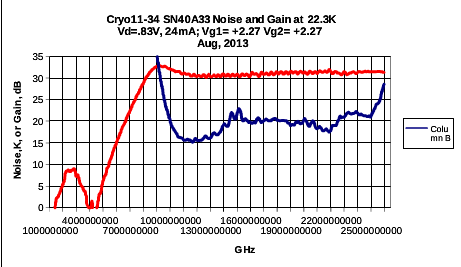
\includegraphics[scale=0.9]{hemt1afterrepairaug}
\caption{Hemt 40A33 Aug 2013 at 23.2 K as measured by Sander Weinreb at Caltech.}
\end{figure}

\begin{figure}
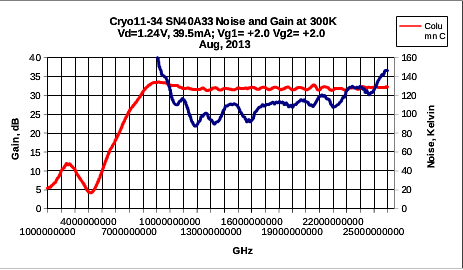
\includegraphics[scale=0.9]{hemt1afterrepairwarm}
\caption{HEMT 40A33 July 2013 at 300 K as measured by Sander Weinreb at Caltech.}
\end{figure}

We measured the noise temperature of the HEMTs plus the waveguides at XX K using a Y-factor measurement to be XX. The two HEMTs have a 3 dB attenuator between them.

The Receiver

The room temperature electronics serve to further amplify, filter, and mix the signal to baseband. 

SCHEMATIC OF ROOM TEMPERATURE ELECTRONICS
\begin{figure}
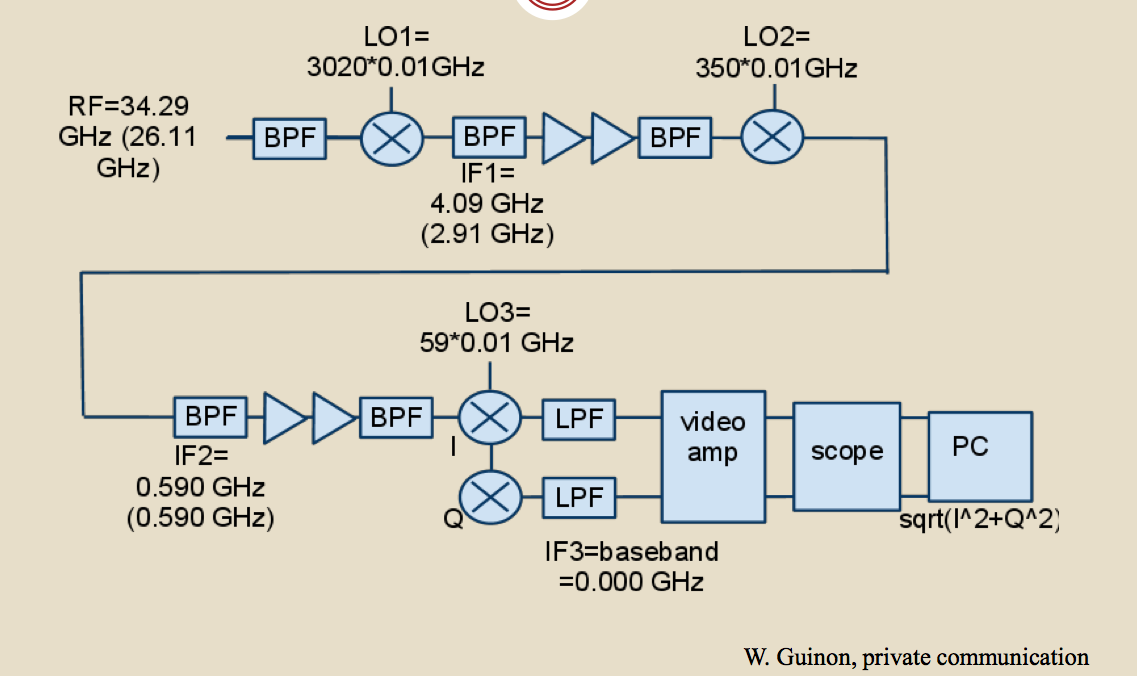
\includegraphics[scale=0.3]{receiverdiagram}
\end{figure}

Put in a table of the gains and noise powers.

TABLE of GAINS and NOISE POWERS
\begin{table}[ht]
\caption{Gain and Noise Power Along Receiver Chain}
\begin{tabular}{c c c c}
\hline\hline
Element & Gain (dB) & Expected PSD & Measured PSD (dBm/Hz)\\ [0.5ex]
\hline
Before 30.5 GHz mixer & x & y \\
After 4 GHz amp & x & y \\
After 4.09 GHz mixer & x & y \\
After 590 MHz amps & x & y \\
After 25 MHz filter & x & y \\ [1ex]
\hline
\end{tabular}
\label{table:gainsofreceiverchain}
\end{table}

There is an RF filter with a bandpass from 32.6-36 GHz. THere is a mixer whose LO comes from the ANRITSU signal generator (so is tunable) with conversion loss XX that mixes the signal to the 4 GHz range. Then there are two cascaded amplifiers in the 4 GHz with total gain 60 dB (and a filter before and after them with width 1? GHz), and second mixer with local oscillator fixed at 4.09 GHz. This mixes the signal down to around 590 MHz. There is then another amplifier with 30 dB gain, and a 25 MHz filter around 590 MHz (again before and after the filter). The mixers are all from MITEQ GET MODEL NUMBERS, as are the amplifiers. The filters are from Spectrum Microwave. The last mixer is an IQ mixer that mixes 590 MHz down to zero. There are two outputs, the I and Q channel, and each has a 4 MHz lowpass filter at the output. THe BNC outputs go to an SRS MODEL NUMBER voltage pre-amplifier, set to 50 ohm input impedance and voltage gain of 5. This then goes to the PCI-5114 digitizer card, which samples at a 10 MHz rate set by the external digital clock.



\section{Experiment}

The experiment of a 7 T NMR magnet and a cryostat in the vertical bore of the magnet. The magnet is in persistent mode, meaning that we only have to fill it with nitrogen and helium periodically. The magnet is from Oxford instruments and has an 8.9 cm diameter. The insert is from Cryo industries and consists of a 1.57" inner diameter, and a nitrogen jacket followed by an insulating space and the enclosed region. The helium reservoirs are located at the top of this dewar and a capillary line feeds through from the helium reservoir to the bottom of the dewar, with a flow valve connecting them.

We place the assembly of the cavity, low noise cryogenic amplifier, and waveguides, which we call the insert, into the cryostat with a vacuum seal at the top. There are several temperature sensors and the power leads for the LNA is also fed through.

A typical cooldown consists of filling the nitrogen reservoir of the cryostat, which we can do automatically through an autofill mechanism, clearing the capillary line from any air or nitrogen by running helium gas through from the helium reservoir, opening the flow valve and pumping on it, and then filling the helium reservoir. To go from room temperature to 4 K at the bottom of the dewar generally takes about three hours. If we do this procedure the night before, when we fill the nitrogen and helium again the next day it only takes an hour, generally.

There is a pump on the inner region of the cryostat, which is a roughing pump. We also have valves that open the inner region up to atmospheric pressure.

I should also mention that the tuning mechanism, which in this case consists of a long rod that is attached at the top via a screw, is coupled in a vacuum compatible way. The waveguide and cavity together consist a closed system - we pump on the waveguides when trying to keep liquid helium from entering the cavity, which it can do most probably through the tuning rod connection. 

The tuning rod connection consists of a bellows which allows the rod to enter a vacuum compatible region that has vertical motion capability.

The tuning rod consists of a G-10 rod, .125" diameter. The waveguides are made of several pieces - at the top of the insert there is a six inch section of stainless steel copper coated waveguide, and the rest is copper waveguide. This is to reduce the heat load on the bottom of the cryostat. The waveguides used throughout are WR28 - which means rectangular waveguide with a lower cutoff frequency of 21.5 GHz.

The cryostat is a gas flow design, meaning the primary mechanism of cooling occurs through convection? Movement of the helium gas from the bottom where it is boiling off from the liquid collected to the top. The atmospheric valve is left open so that when running the cryostat has slightly more than atmospheric pressure. There are several circular mylar baffles in place as well.

The pump on the waveguide is also a roughing pump. At room temperature the vacuum sustained is roughly 30 millitorr, although the pressure sensor does not go below this value, so it may be lower. In any case, when we cool down due to cryopumping the vacuum in the cavity region, assuming no vacuum leak, should be very good.

The temperature sensors go to a computer which logs the data.

\section{Electronics}
\subsection{LNAs}
The electronics for measuring the RF signals consist of a series of amplifiers, mixers, and filters. The first element of this chain are the low noise amplifiers. These are placed in the cryostat and are High Electron Mobility Tranisistors. We have two, with a three dB attenuator between them. The first amplifier (both were ordered from Sandy Weinreb at Caltech) was measured by him to have a minimal noise temperature of 22 K at 20 K and 34.3 GHz, and a noise temperature of 210  K at room temperature. Check this. The second amplifier has slightly worse characteristics - the noise temperature at 20 K is given as 30 K and at room temperatue it is 400 K. The gain given by Sandy Weinreb is 29 dB for the first and 30.5 for the second, which we measure to be the case at room temperature.

Put in the S. Weinreb measurements here

Put in the VNA screenshot of the amplifier gain at room temperature here.

\subsection{Rest of Electronics}

The next element in the electronics is a waveguide filter which has a passband of 32.6 to 36 GHz. After that is a waveguide to coax adaptor (I should mention that these elements are also at the input and output of the double HEMt assembly) and from there we can attach mixers or the VNA cable.

The signal coming out before the mixer is usual -143 dBm/Hz. Since the noise floor of state-of-the-art spectrum analyzers is -155 to -160 dBm/Hz this is very close to the noise floor. At the time of writing, we implemented our own home made spectrum analyzer which consisted of two parts - an analog mixing sequence that physically mixed (and amplified) the signal down to baseband frequencies and suppressed image frequencies - the mixing is in order to reduce the amount of data we have to acquire, and once the signal is mixed down a computer computes the Fourier Transform, the square of which is the power spectral density. The Fourier Transform is computed using the FFTW libraries. FFT, or the fast fourier transform, is an algorithm for doing fast computations. I am not sure how it works.

The details of the mixing sequence are as follows: the first mixer has an LO input from a signal generator that can give out signals at frequencies up to 40 GHz. We usually set the LO to 30.2 GHz for RF signals to the input of 34.29 GHz. This would make the intermediate IF frequency around 4.09 GHz.There is then 60 dB of amplification and further filtering before the second mixer, which has a fixed LO frequency of 3.5 GHz. The IF then becomes 590 MHz. With more filtering and another 30 dB of amplification the 590 MHz signal enters an IQ mixer, which separates the in phase and quadrature components of the signal and mixes both down to baseband. There are two 25 MHz (or 4MHz) filters on the I and Q outputs, which determines the final bandwith of our home made analyzer.

All these elements are commercial and from MITEQ. The reason for filtering is to suppress image frequencies (frequencies $f_{image} = f_{LO}-f_{IF}$) since there are two frequencies that can mix down to the same intemediate frequency. The reason for the particular values of the local oscillator frequencies is that they are all multiples of 10 MHz so they can be all phase locked with a 10 MHz reference clock (in this case the clock is from the Anritsu signal generator) and the reason for the three stages of amplification is that these components seemed like a good idea.

The output power of the I channel after going through a voltage pre-amplifier (which turns power into voltage don't ask me how) is -97 dBm/Hz when looking at the thermal noise of a ~5 K cavity before the LNAs. The output power of the Q channel is usually -96 dBm/Hz. The difference between them are due to imperfections in the I/Q mixer.

After getting the voltage amplified by a factor of 5 in the pre-amplifier (SRS 5330?) the two channels are digitized by a National Instruments high speed digitizer, which is also fed the 10 MHz reference clock. We then Fourier transform the time domain data to obtain the spectral profile.

\begin{figure}
\centering
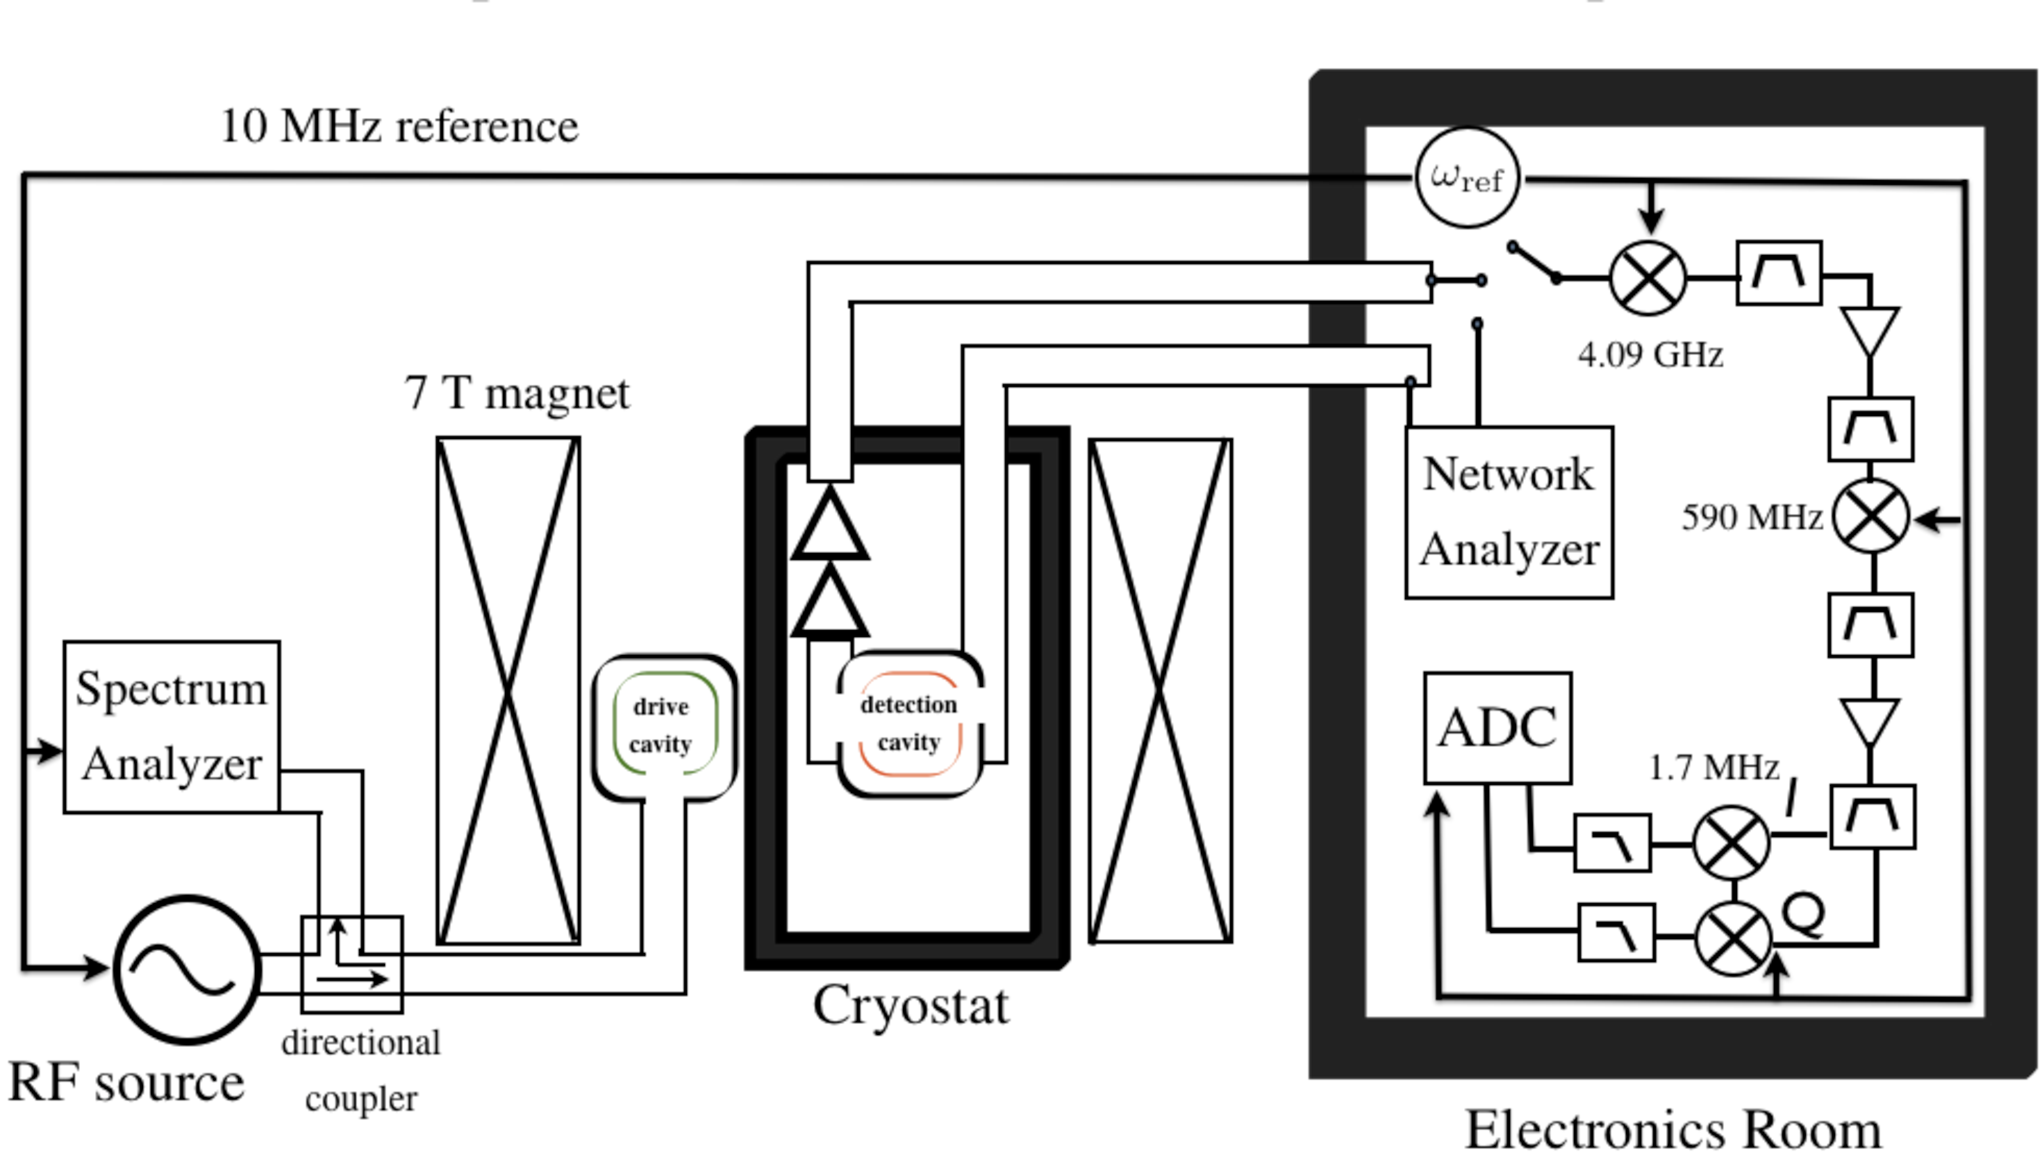
\includegraphics[scale=0.35]{malagon_ana_fig1}
\caption{Schematic of the experimental set-up. The intermediate frequency at every stage of the receiver chain is shown, along with the amplifiers and filters.}
\label{fig:schematic}
\end{figure}

\section{Data}

To date we have performed two experiments - one using a single "quiet" cavity in the magnetic field, cooled to 4 K, and one using two cavities, with one quiet cooled cavity and the other driven by an RF source.

The first experiment looked at the TE011 resonance (tunable but centered around 34.29 GHz) and tried to set a limit on the possible scalar particle-photon couplings that this setup could potentially detect. The starting assumptions are that the dark matter halo has a density of these scalar particles given by  $10^{13}$ GeV/${cm}^3$ which acts as the initial seed for these particle-photon conversions. The reason photon-particle conversions are not seen as a cancelling effect is that the number of photons is so much less than the number of particles that we have a huge population inversion $n_{ALP} >> n_{\gamma}$, and also that these conversions are so rare that a particle-photon-particle conversion and then reconversion would be suppressed by an extra factor of the weak coupling.

The particle-photon conversion is stimulated by the presence of the strong magnetic field and enhanced in the region of a cavity, since there are fewer states that a cavity can support, therefore by Fermi's golden rule the transition probabilities of going from this continuum particle state to the discrete mode state of the photon are higher. This is known as the Purcell effect when talking about enhancement or suppression of spontaneous emission of an atom in a cavity.

So the expression for the probability of conversion goes as the number of particles available to emit a photon (nV), the probability of a single particle conversion in free space with a magnetic field $(gB)^2$, the overlap integral expressing how likely the emitted photon is to be in the particular mode j we measure $(f_{j})$, and the enhancement by the Q of the cavity (Q). By conservation of angular momentum the emitted photon must have the same polarization as the magnetic field (really this is a two photon interaction, with the magnetic field providing a "virtual" photon), so since the magnetic field is axial, for a scalar interaction the emitted field must be a $TE$ mode (meaning the only axial field is magnetic, not electric).

Therefore we have $P_{a\gamma} = (gB)^2 nfVQ.$ If the density is, as commonly the case, written as the energy density and not the number density we have $P_{a\gamma} = (gB)^2 n_e f_{j} VQ/m_a$, where natural units are assumed.

Unfortunately the problem with looking for particles that give off photons whose wavepacket overlaps in a non-zero way with the $TE_{011}$ mode or in fact any $TE$ mode is that due to symmetry considerations, the overlap integral is in general very small or zero. The reason is because of boundary conditions -by Maxwell's equations the incident normal B field on a conductor must be zero, so for the axial magnetic field $B_z$, the boundary conditions imply $B_z(z=-L/2)=B_z(z=L) = 0$ so all $TE$ mode have an even $B_z$ field around $z=0$. But because of cylindrical symmetry, the value of $B_z(z,r=R)$ must be the same at diametrically opposed sides of the cylinder (at least for the lowest order mode). Because there are no magnetic monopoles, the magnetic field must integrate to zero. 

As well, I was lying when I said $f_j$ goes as the integral of $B_z$. If you go through the equations of motion for Maxwell's equations with a source term of the form $B_z\cdot B_{magnet}$, the source term is actually second order with regards to $g$.

Both of these things make it extremely hard to detect scalar particles in microwave cavities due to symmetry considerations and magnetic field properties.

We nonetheless performed the experiment and were able to exclude $g > 10^{8}$ 1/GeV for masses $~0.14$ meV.

The second experiment performed was for a two cavity detection method. Here the photon-particle-photon process is employed. By using an RF source as the photon source, we hope to produce these weakly interacting particles. Applying conventional shielding (any material) will attenuate the photons but not the particles. However to detect them we need to convert them back to regular photons. Since this process involves to extremely rare events, it suffers from the $g^4$ factor, but with a high intensity source of photons and using enhancement of the generation and detection volumes, one can improve the sensitivity to make experimentally interesting measurements. One caveat - having a high Q in the detection region will enhance sensitivity due to the Purcell effect as discussed above, but the Purcell effect is not what allows us to get enhancement by Q in the generation region. This is just due to the fact that the power in a cavity scales as the input power times Q.

Instead of $f_j$ we now have $G$, the geometry factor, in the probability of this process occurring. $G$ takes into account the modes of each cavity and the distance between them.

For vector particles, $G ~ 0.12$ for two $TE_{011}$ cavities separated by 3 cm. For scalar particles $G = $ I don't know for scalars, probably zero since the generation probability is zero. And of course zero for pseudoscalars which need a different polarization of the mode, since we were only looking at the $TE$ mode. However maybe it is non-zero for another mode.

For this two cavity experiment, we drove one cavity $TE_{011}$ mode with a signal generator set for its maximum stable output of 22 dBm or 158 mW. The signal was a cw signal at the cavity resonance, usually 34.299 GHz, although it changed by about 300 KHz due to variations in room temperature. The bandwidth of the signal is very small, about 0.1 Hz. There was approximately a meter of waveguide between the cavity and the signal output, as well as a directional coupler and isolator between the two. At 34 GHz the loss of wr28 is 3 dB/m, and since the cavity was observed to be not critically coupled, there is probably more than 6 dB of power that does not get into the cavity. This changes the power entering the cavity to about 16 dBm, or around 30 mW. For a Q of  around 7,000,  this means that the power circulating in the cavity is in general around 210 Watts. Is this right? I am not sure, it seems to be wrong. Need to look at accelerator books and people who talk about RF power.

As the cryostat is in the bore of the magnetic field, the driving cavity is also placed in the bore, next to the cryostat. Thus the walls of the driving cavity, the cryostat walls, and the walls of the quiet cavity all act as layers of attenuation for regular photons. We cool the quiet cavity down to 4 K to reduce the background thermal noise, and encase the electronics for mixing and analyzing the RF signal in a metal room which acts as a Faraday cage to close off any potential interference from the 22 dBm source.

Our first measurements showed that there was an intermittent signal at our frequency of interest on the level of 3 dB above the thermal noise background. We had the driving cavity detuned with respect to the driving frequency $\omega_L$, so the observed spike, if from hidden photons would have to come from a process whith only one Q and a much lower G, since it would have to convert from the circular mode of the waveguide which connects to the cavity. So by suppressing any possible $\gamma'\rightarrow \gamma$ conversions, we test for interference exclusively. When the quiet cavity and driving cavity were retuned, the leak appeared to be larger, but still intermittent. We suspected that the interference was happening in the electronics, not through the cryostat or cavity. Two suspects were the power leads for the LNAs that could carry an RF signal down into the cryostat or the various connections in the mixing scheme which could pick up EM leakage. At room temperature with the LNAs powered off, the spike was observed but disappeared by closing the door to the shielded room encasing the electronics. At room temperature with the LNAs powered on ... this has not been tested.

With the parameters in our setup we were able to place an exclusion limit on the coupling of vector particles to photons for $\chi > 10^{-7}$ 1/GeV.

\section{Cavity}

The cavities we use for detection are made to resonate at frequencies near $~34$ GHz. This choice has to do with the predictions for the resonant frequency of axions, sensitivity, and the constraints on making 3D cavities that will fit into the space limitations of our current setup.

Taking the most practical consideration, the diameter of cavities scale in size as $\lambda$. We assume throughout we are only interested in low order modes for which the prefactor for lambda is O(1). If we wish to tune the resonant frequency of a particular mode, the common methods are perturbing the cavity geometry, either by inserting a dielectric or physically changing the size of the cavity. 

For axion searches, only $\text{TM}_{0n0}$ modes couple to the emitted photon, and the frequency is independent of the cavity height, which is easier to adjust than the radial dimension. Therefore the scheme that we use for our $TE_{011}$ cavity of using a floating cap that we can vary the height of (called the plunger) no longer works.  

So instead we change the effective velocity of light in the medium by introducing a dielectric, in our case alumina ceramic which has a relative permittivity of $\epsilon \approx 9.3$. The size of the dielectric will affect how much it perturns the cavity mode - in our case we limited the size of the dielectric rod by considering what the cutoff frequency was of the tube in which the dielectric was held. For a circular tube (which is essentially a waveguide) with $\epsilon = 9.3$, light will not propagate until 35 GHz (check this) for a diameter of 0.063". The alumina rod is from McMaster-Carr with the parent company being Coorstek. 

In order to keep the mode Q high, it is best not to destroy the axial symmetry of the $TM_{0n0}$ mode so we insert it vertically in the center. It is also easier to make vertical insertions that horizontal ones, where the cavity must be aligned with its axis along the axis of the magnet. 

Not only the resonance frequency, but the overlap integral $f_j$ will be affected by the dielectric since the fields in the mode are perturbed. Other groups (ADMX) have seen that inserting a dielectric rod can cause large degradation in the field mode, however we do not find this to be the case in our simulations for the range of insertion depths tested.

The cavity coupling holes are two. The first one is to couple power out of the cavity. For critical coupling, the power coupled out is equal to the power lost in the walls. This gives optimal signal to noise. The other hole is so that we can send in power in order to do transmission measurements, which allow us to determine the Q of the cavity and the resonant frequency. This hole is in general very weakly coupled (we estimate it to be around ~-46 dB). 

We use coupling holes instead of antennas for god knows why. The reason is at the frequency we work at it is problematic using cables. They are lossier than waveguide and I don't know what else.

The cavity coupling hole is simulated as a stretched circle (meaning it can be viewed as a hole constructed as the sum of two circles whose centers are offset from each other by some distance and a rectangle in the center whose length is that same distance). We try to couple to the magnetic field of the waveguide in the TM020 mode and in the TE011 mode. There is no intrinsic advantage to this, just that the geometry of the fields in the waveguide and in the cavity and our space constraints make it easier to have vertical waveguides on the sides of the cavity and the fields in the mode that align with the propagating fundamental mode of the waveguide happen to be magnetic ones.

The next thing to talk about is that the cavity in the TM020 mode must have good connection between the walls and the caps because the alternating E field means that there are vertical currents that switch direction and flow in the vertical axis so if they cannot flow to the top or bottom cap, the mode's Q will be severely degraded.

The reason we have been talking about TM020 all this time is because the Tm010 mode has too small a size in the 34 GHz range. Let us expand our range and take the entire Ka-band, or R-band as it is sometimes called. From 26.5-40 GHz, if the Tm010's resonant frequency lies in that range, it's cavity radius would be 4.33 mm to 2.869 mm. Hmm that actually seems pretty ok for the lower range. Why are we workign at 34 GHz anyways? The Tm020 mode would have 9.9mm-6.58mm. The size of our current opening in the cryostat is 40 mm. Our current cavity has a radius of 5 mm in the Te011 mode.
However! We believe that the TM020 mode has a higher Q, at least theoretically, which with the higher volume for the same frequency, actually compensates the degraded C (C for 010 is 0.69 and C for 020 is 0.13). Although there are more mode crossings, we don't worry about this because we make the cavity height sufficiently small so that other modes can't come in.
The reason we are working above 20 GHz is because this region is as of yet unexplored. People have been using large microwave cavities to look for lower mass axions because of the higher sensitivity due to the large volume. It is our goal to push the exploration to higher masses in order to investigate possible axion-photon couplings in this as of yet unexplored region.
The reason we are working precisely at 34 GHz is pretty stupid though. We wanted to use a high power pulsed source which puts out fixed frequency 34.29 GHz radiation. Then we designed our whole system around it and now don't want to change it because it would be a pain.
Our other limitations are the present waveguides installed (fundamental mode operates between 21.5 and 40 GHz even though the rating says 26.5-40 GHz) and the RF filter. Also our electronics might not be happy. But the LNAs can go from 11-34 GHz.
We mention here that we are tryng to do something that cavities are not really made to do - be a broadband detector. They are very good at picking out specific frequencies from a broadband input, or enhancing processes when the radiation these processes emit is at a frequency where the cavity resonates. So much work is being done trying to bring tuning, which is a slow process with a cavity, into the picture.
Maybe some ideas would be trying to use metamaterials or do mode-locking somehow. I don't think our amplifiers have the bandwidth to support more than two, maybe three modes mode-locked and I haven't seen anything that says that people have tried to mode-lock microwave cavities, but this woud emit radiation at higher peak intensties because they would all be emitted in one short burst. I thought this would improve our 
signal to noise but maybe it wouldn't because we only care about fluctuations in the signal and these are not different are they? I don't know.
Also a way to get around the high frequency, small volume problem seems to be to make it not be a problem - ie find ways to make high volumes resonate at high frequencies in low order modes. So we need an anti-dielectric, which will increase the frequency rather than lower it. Dielectric smaller than one only exist as things called metamaterials and I don't know their RF properties.
Or maybe mode-locked detectors could help us because of the thing of pulsed things having better signal to noise than cw things. Not really sure.


\section{Receiver Noise Figure}

Because of the Friis formula the noise in the entire electronics analyzing chain is dominated by the noise of the first amplifier if it's gain is high enough.

\section{HSP Introduction}

We also did a HSP search using two $\text{TE}_{011}$ cavities. There was one $\text{TE}_{011}$ cavity that was not tunable and had a resonant frequency of 34.29 GHz. It had one aperture coupling on the bottom face where it went to 13 mm cylindrical waveguide and then to WR28. There was a meter and a half of this between an isolator and directional coupler and before all of that a signal generator capable of putting out 25 dBm but in practice we operated it at 22 dBm because it would output a warning that the power was unleveled at 25 dBm. 

There the reflected power went through the directional coupler to a spectrum analyzer.

The $\text{TE}_{011}$ cavity (signal cavity I’ll call it) was inside the bore of the magnet but outside the cryostat

SHOW SCHEMATIC OF EXPERIMENT

EMI Shielding

There are many shielding improvements made iteratively. I list them below:

1. Aluminum Wool in Bore of Magnet
2. Copper Tape Over Joints of WR28 connections
3. Copper tape over Vacuum Tube connections in Shielded Room
4. Terminator on Cable to Weak Port when Disconnected
5. HEMT power supplies moved to different room than both magnet and shielded room
6. Everything locked to 10 MHz reference
7. Shielded Room Shut and Run on Battery Power
8. 10 MHz BNC cable hole drillled in shielded room wall and had RF absorbing foam placed around opening
9. Aluminum Wool Placed in Holes leading HEMT power supply cables out.
10. One HEMT power supply grounded through another HEMT power supply.

\section{Expected Sensitivity}

As the power is monochromatic, by reducing the resolution bandwidth we decrease the noise in each bin while the power stays the same. The size of each resolution bandwidth is inversely proportional the number of samples we acqure, and thus the integration time. The exact formula is 

resBW = 1/tau

When no windowing is used.

\section{Thermal Noise - As Expected?}

\section{Hypothesis Testing}

\section{HSP Results}

Hopefully we can redo these results, but we were able to make an exclusion based on non-observation of a peka in a 2.5 minute run.

\begin{figure}
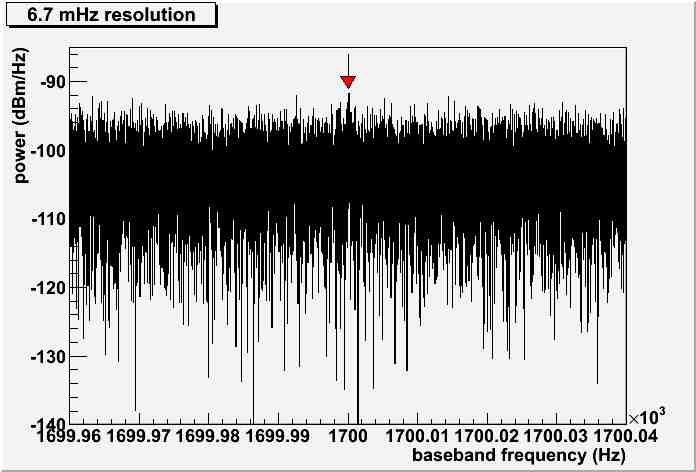
\includegraphics[scale=0.3]{malagon_ana_fig2}
\end{figure}
\begin{figure}
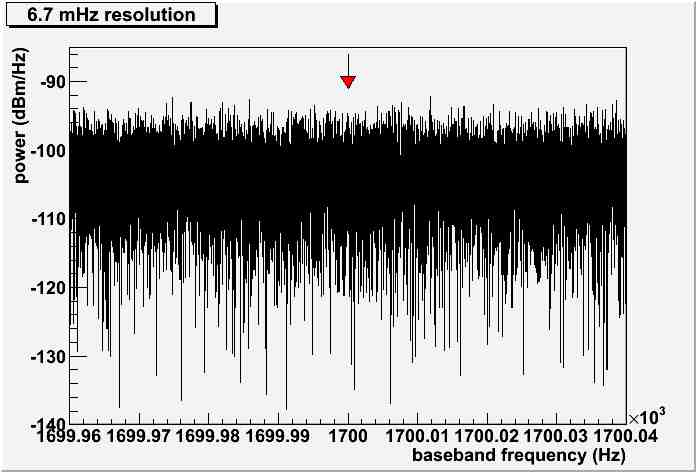
\includegraphics[scale=0.3]{malagon_ana_fig3}
\end{figure}

\begin{figure}
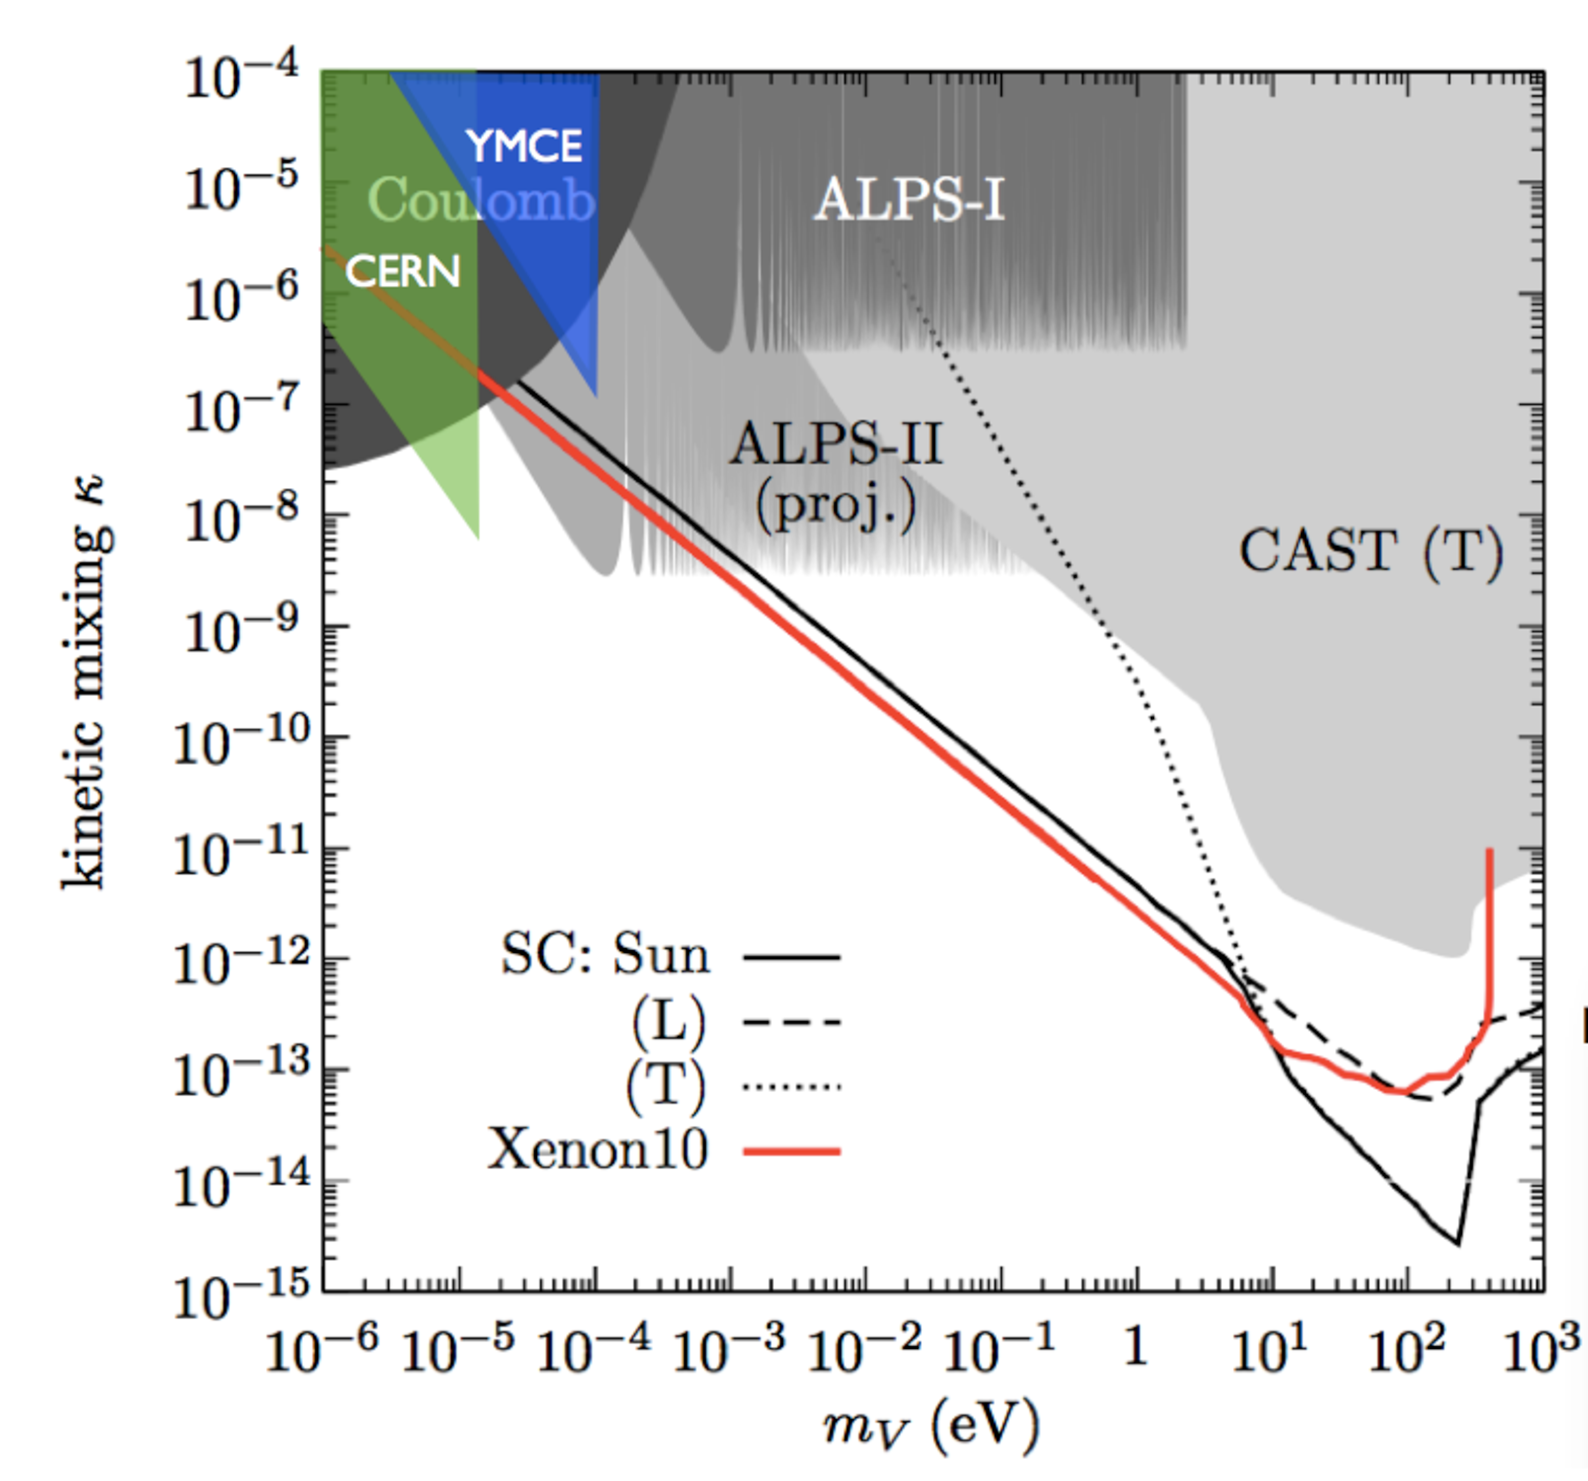
\includegraphics[scale=0.3]{malagon_ana_fig4}
\end{figure}

\end{document}